\section{Bioshock}

\begin{figure}[htbp]
\begin{center}
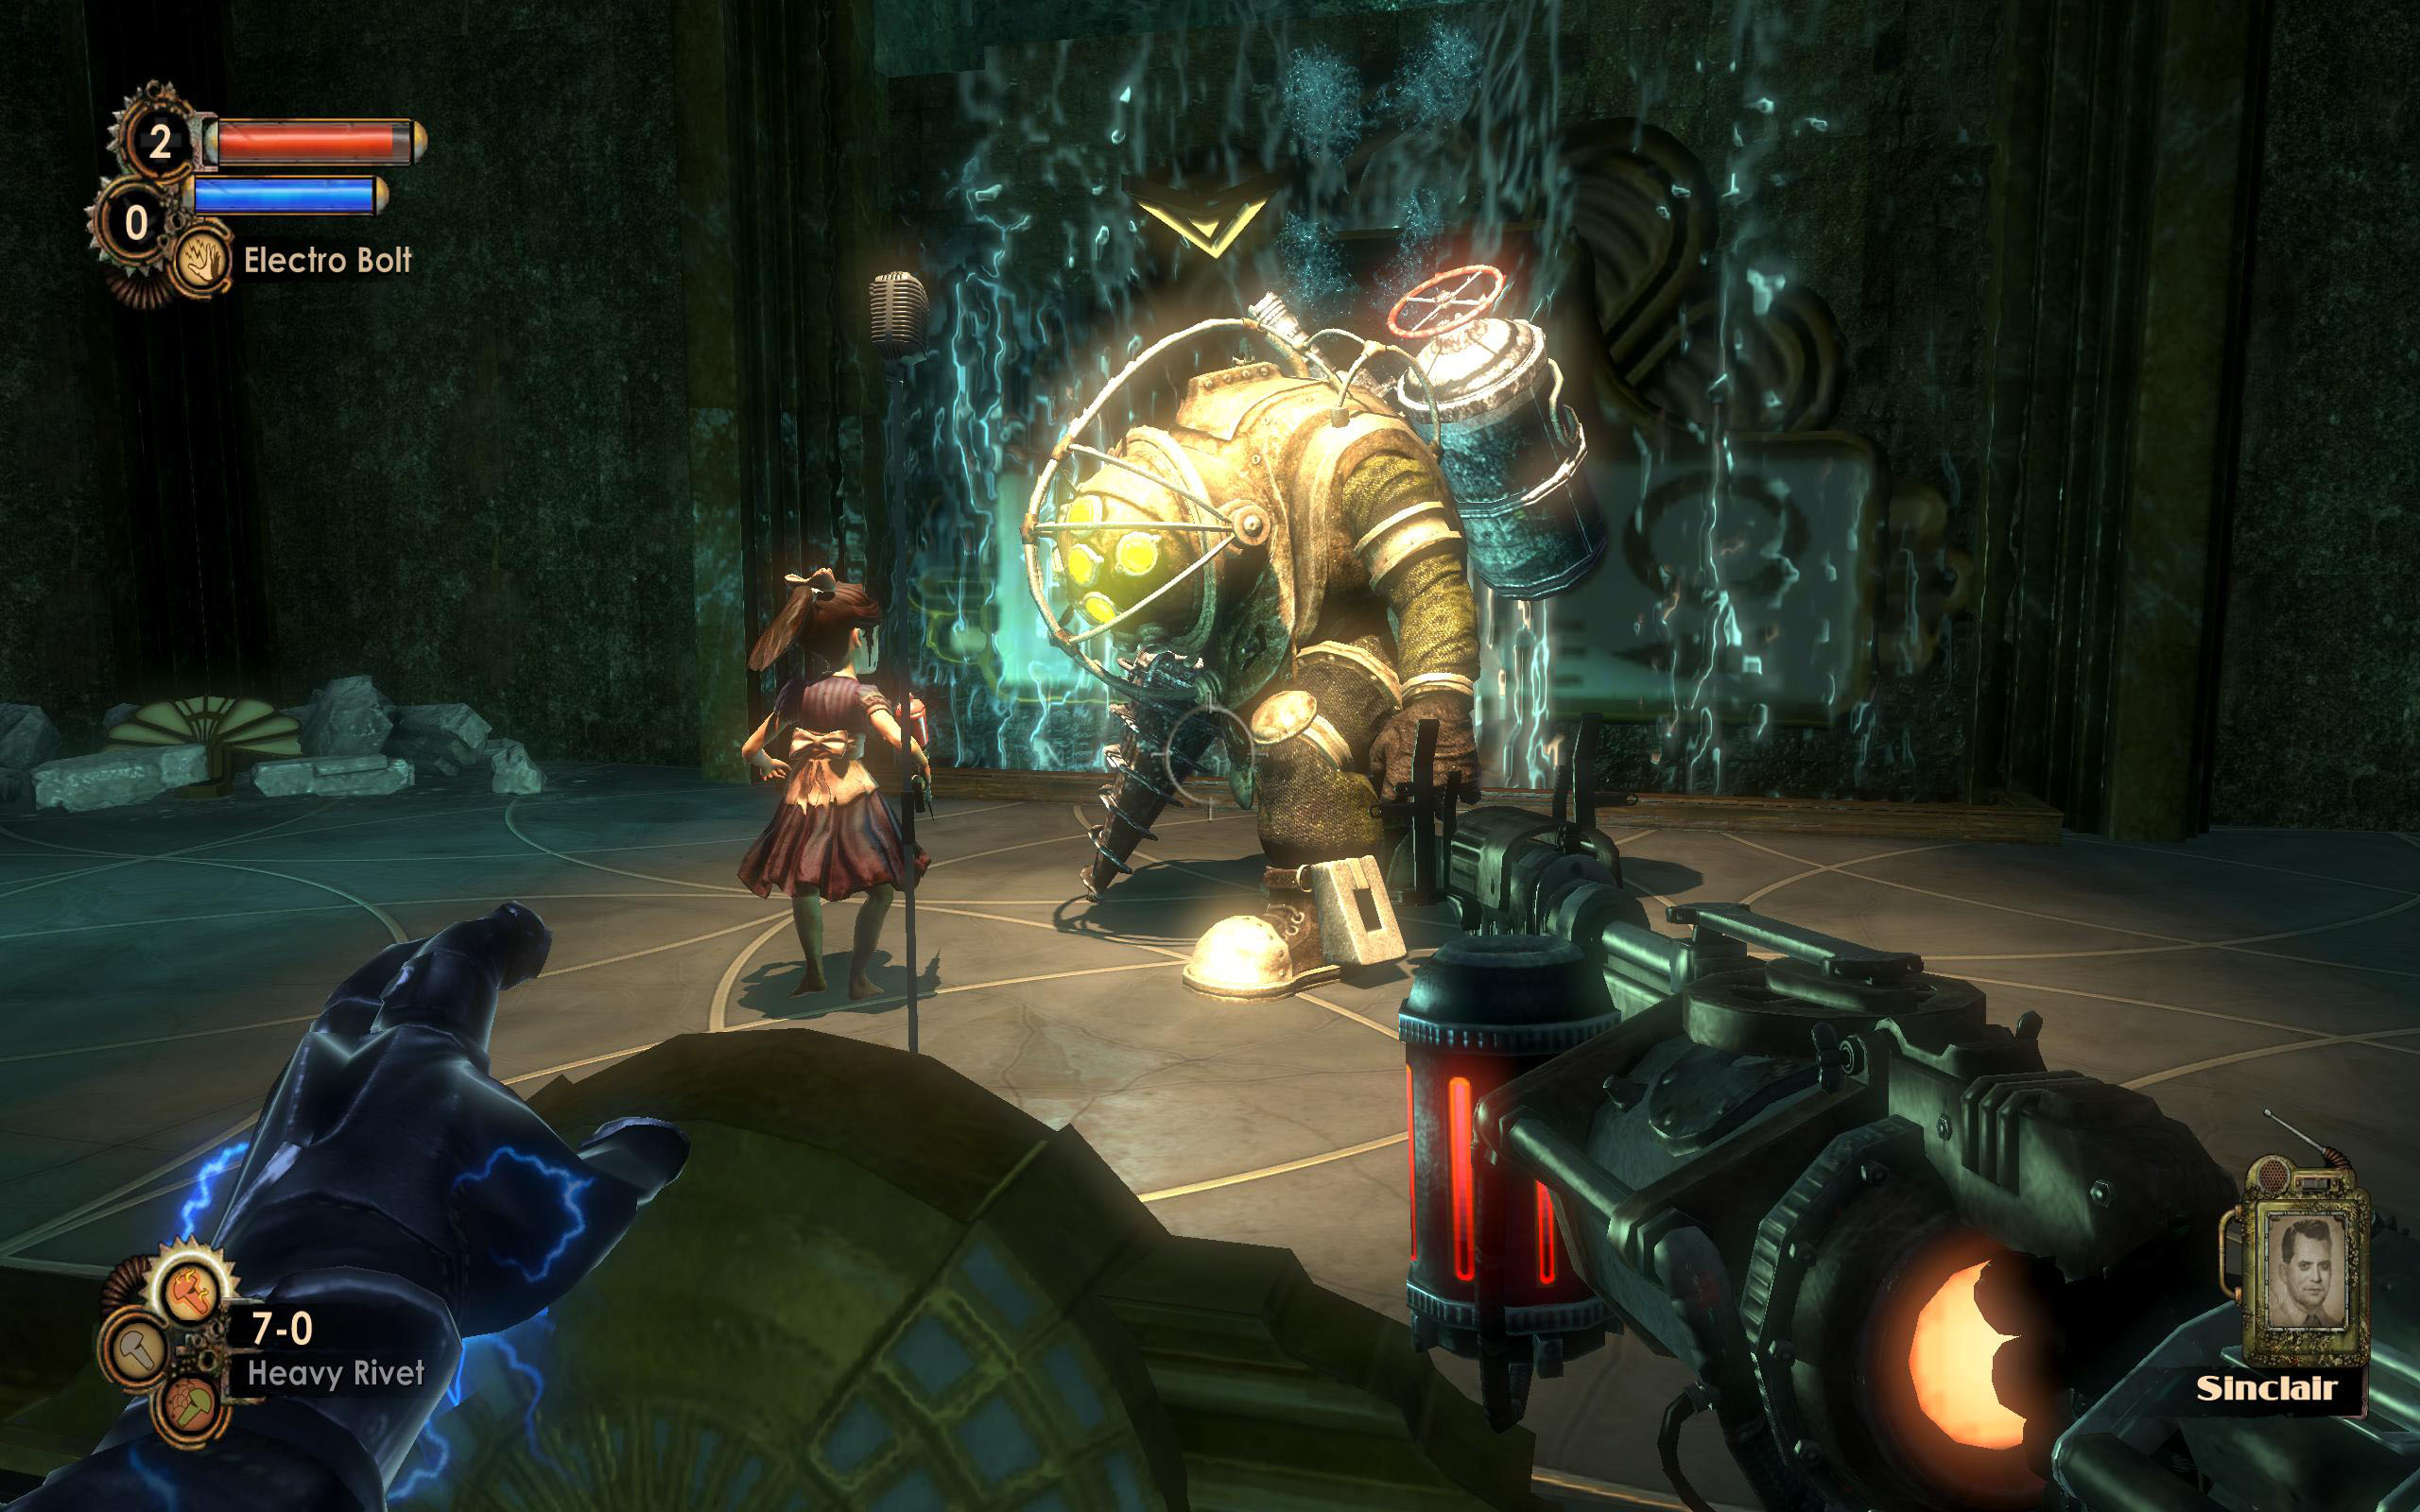
\includegraphics[width=.60\textwidth]{./imagenes/bioshock.jpg}
\caption{Bioshock}
\label{Bioshock}
\end{center}
\end{figure}
Bioshock\footnote{\url{http://http://www.bioshockgame.com/}} es un juego de disparos en primera persona desarrollado por Irrational Games.

El protagonista, luego de caer al océano debido un accidente aéreo, llega a una ciudad submarina llamada Rapture. Construida por un magnate de negocios con el objetivo de llegar a ser una utopía aislada, regida únicamente por los principios filosóficos libertarios seguidos por el magnate. ``Ni Dios, ni reyes. Solo el hombre'' se puede leer en un gran letrero a la entrada de Rapture.

Sin embargo, al llegar, ya es una ciudad fantasma cayéndose a pedazos, con las pocas personas que quedan completamente locas, y la mayoría siempre en busca de una dosis de una droga energética desarrollada en Rapture.

El jugador se debe abrir camino utilizando armas e inyecciones para alterar su genética, además de tener que hackear algunos dispositivos para poder obtener comida y municiones.

\subsubsection{¿Por qué es uno de mis juegos favoritos?}
\begin{itemize}
\item[Ramón Carrillo] No solo es un juego de acción, el elemento más destacable es la historia y la profundidad de los personajes, se discuten aspectos morales, religiosos, políticos y filosóficos. La intriga está presente todo el tiempo: ¿cómo se construyó la ciudad?, ¿cuál fue la motivación?, ¿qué hizo que fracasara?, ¿qué pasó con sus promotores?. Y finalmente el aspecto retrofuturista de Rapture y los sonidos que provienen ya sea de un robot o de otro esquizofrénico habitante lo convierten en un juego que atrapan tu concentración totalmente.
\end{itemize}
